\section{Conceptual Modelling}\label{sec:cm}
%Conceptually model your database using an E-R diagram. Use the legends in your diagram. Write how you find the entity types, relationships, and attributes from Section~\ref{sec:rga}
\textbf{ER} Diagram stands for Entity Relationship Diagram, also known as \textbf{ERD} is a diagram that
displays the relationship of entity sets stored in a database. In other words, ER diagrams help to explain the logical structure of databases. ER diagrams are created based on
 three basic concepts: entities, attributes and relationships.
 \begin{enumerate}
    
\item Entity type: A group of definable things, such as User, whereas the entity would be the specific User. 
\item Entity set: Same as an entity type,but defined at a particular point in time, such
as User registration first day of the month.
Relationship: How entities act upon each other or are associated with each other.
\item Attribute: A property or characteristic of an entity. Often shown as an
oval or circle.
\item Cardinality: Defines the numerical attributes of the relationship between
two entities or entity sets . The three main cardinal relationship are (1).one-to-one,(2). 
one-to-many and (3).many-to-many.\\
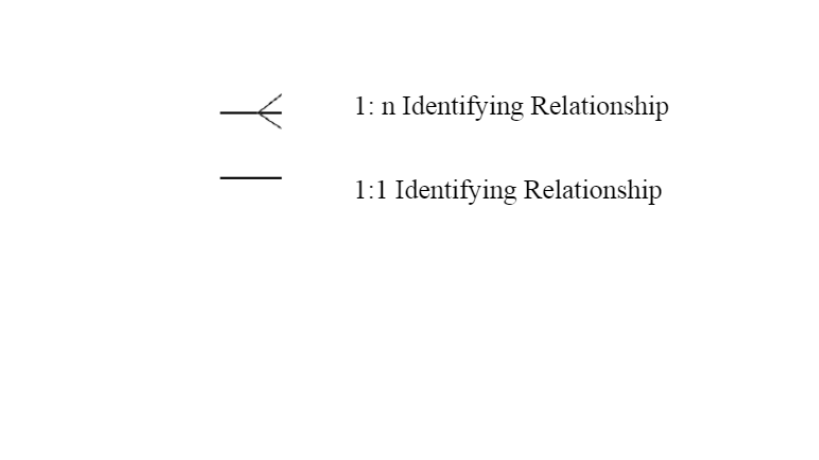
\includegraphics[width=1\textwidth, inner]{relationship.png}\\
According to requirements, we have to store about the admin, flat-owner, flat, facilities and renter. Finally, we find here 5 entity types like General User, Flat Owner, Admin, Flat, Facilities.

    

%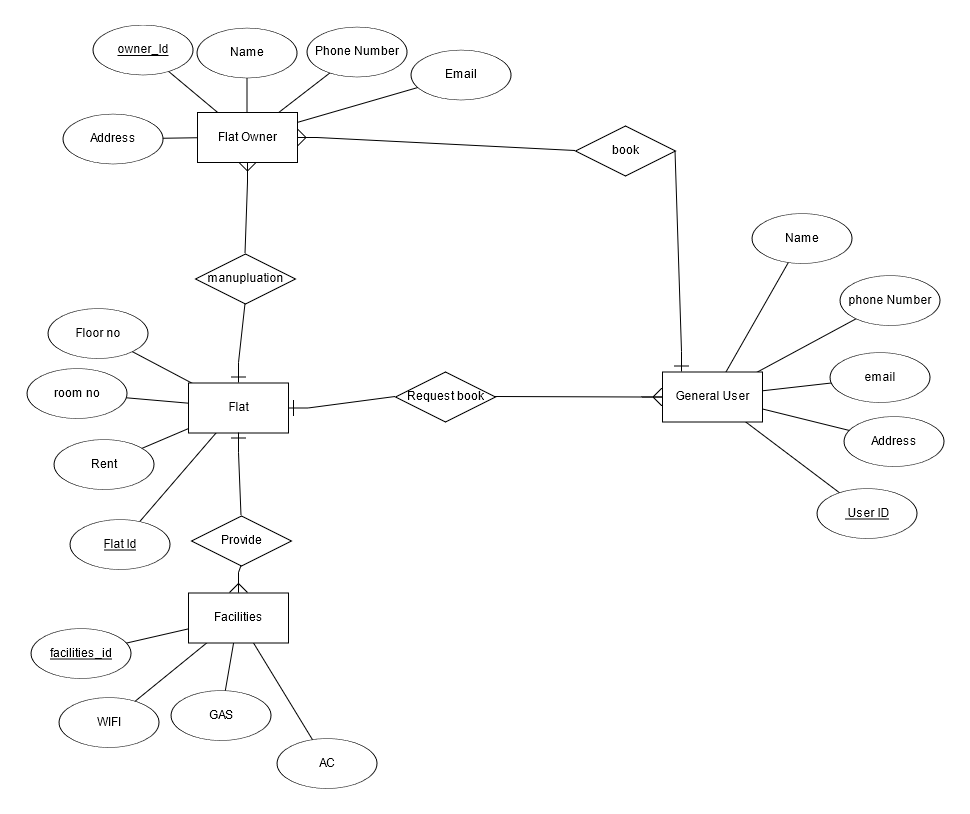
\includegraphics[width=1\textwidth,inner]{images/erdiagram.png}\\
%\begin{center}
   % Fig 1.1:ER Diagram
%\end{center}
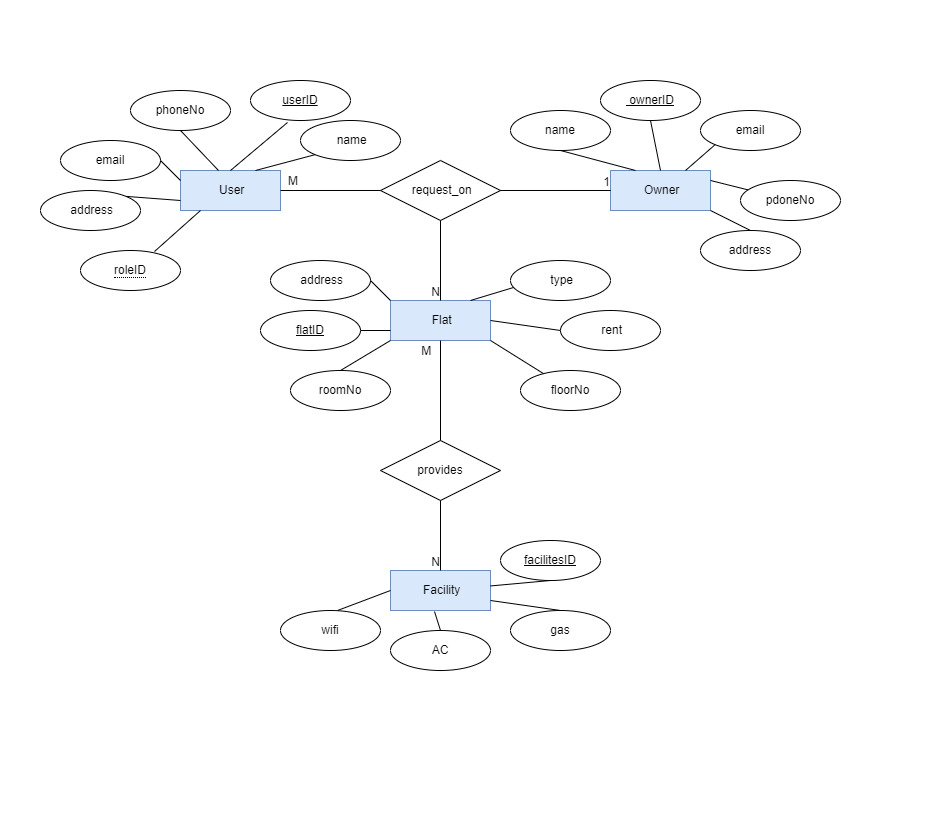
\includegraphics[width=1\textwidth,inner]{images/_erd.drawio.jpg}\\
\begin{center}
    Figure-1: Entity Relationship(ER) Diagram.
\end{center}
 
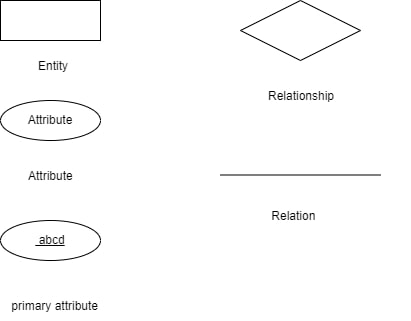
\includegraphics[width=1\textwidth,inner]{images/_ Legends used for ER diagram01.drawio.jpg}\\
 \begin{center}
    Figure-2: Legends used for ER diagram.
\end{center}


 \end{enumerate}    
 \\
 \\
 \newpage
 \noindent
 \textbf{Unary relationship (recursive):}
A unary relationship, also called recursive, is one in which a relationship exists between occurrences of the same entity set. In this relationship, the primary and foreign keys are the same, but they represent two entities with different roles.
 \\
 \\
 \textbf{Binary relationship:}
 When there are exactly two  entity sets participating in a relationship then such type of relationship is called binary relationship.\\
 \\
 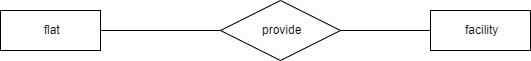
\includegraphics[width=1\textwidth,inner]{images/Binary relationship.drawio.jpg} 
 \begin{center}
    Figure-2.1: Binary Relationship.
 \end{center}
  
 \\
 \\
 \noindent
 \textbf{Ternary relationship:}
A ternary relationship is an association among three entities. This type of relationship is required when binary relationships are not sufficient to accurately describe the semantics of the association. The ternary relationship construction is a single diamond connected to three entities as shown in Figure2.2.\\
 \\
 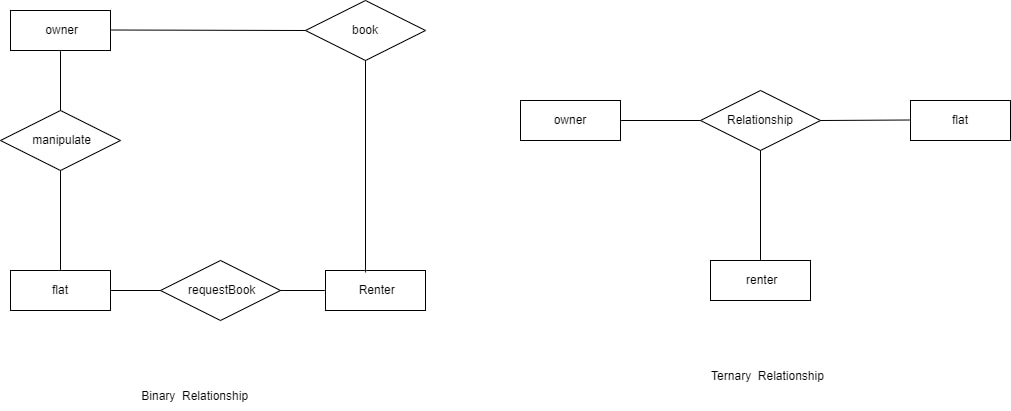
\includegraphics[width=1\textwidth,inner]{images/Untitled Diagram.drawio.jpg}
 \begin{center}
     Figure-2.2: Ternary Relationship 
 \end{center}
 
 
  